\documentclass{article}

% Official NeurIPS 2023 style. The preprint option displays author names.
\usepackage[preprint,nonatbib]{neurips_2023}
\usepackage[utf8]{inputenc}
\usepackage[T1]{fontenc}
\usepackage{amsmath,amssymb}
\usepackage{booktabs}
\usepackage{graphicx}
\usepackage{microtype}
\usepackage[hidelinks]{hyperref}
\usepackage{xurl}

% Identify this document as a course report, not a NeurIPS submission.
% The official style file, font sizes, and margins are unchanged.

\title{Predicting NFL Player Trajectories\newline with Temporal and Interaction Modeling}

\author{%
  Chenyang Zuo \\
  \texttt{2026312303}
  \And
  Zihang Rui\\
  \texttt{2026312268}
  \And
  Hongzhou Zhu\\
  \texttt{2026312302}
}

\begin{document}
\maketitle

\begin{abstract}
Predicting where players move once a pass is airborne is useful both for studying
receiving routes and defensive coverage and as a structured regression problem in
which the future depends on recent motion, nearby opponents, and the intended
destination. We study player trajectory forecasting on the Kaggle NFL Big Data
Bowl 2026 -- Prediction dataset, conditioned on the landing point and horizon the
competition supplies. This report covers the completed mid-term milestone: we
confirm the data and the evaluation split, audit the released files, and implement
both baselines from the proposal. Constant-velocity extrapolation reaches a
validation RMSE of 1.645 yards; a gradient-boosted residual model over 127 features
reaches 0.751 yards, a 54.4\% reduction, stable to 0.002 yards across three seeds.
Feature-group ablations locate the sources of that gain: the supplied landing point
dominates (removing it costs 0.250 yards), explicit player-interaction features
contribute 0.014 yards, and history beyond a short window is largely redundant
(0.022 yards). Error analysis shows the remaining loss concentrates on long horizons
and on coverage players distant from the landing point, and that it is essentially
unbiased, so it reflects route uncertainty rather than a correctable skew. We report
these findings together with the audit caveats that bound their interpretation, and
set the design constraints they imply for the temporal and interaction model of the
next milestone.
\end{abstract}

\section{Introduction}

Predicting player movement is useful for studying receiving routes and defensive
coverage. It is also a structured regression problem: future motion depends on a
player's recent movement, nearby opponents, and the intended destination of the
pass. Constant-velocity extrapolation provides a simple starting point, but cannot
represent changes of direction or responses to other players.

We select \emph{NFL Big Data Bowl 2026 -- Prediction}~\cite{competition}. The task
is to predict designated players' two-dimensional trajectories after the pass is
thrown, using pre-pass tracking data and the supplied play context. Tracking is
sampled at 10~Hz. Let $\mathbf{X}_{p}$ denote the observed features of players in
play $p$, and let $\mathbf{c}_{p}$ denote the supplied context. For each designated
player $i$, we learn
\begin{equation}
 f_{\theta}(\mathbf{X}_{p},\mathbf{c}_{p},i,t)
 = \widehat{\mathbf{r}}_{p,i,t}\in\mathbb{R}^{2},
 \qquad t=1,\ldots,H_{p,i},
\end{equation}
where $H_{p,i}$ is the requested prediction horizon and
$\mathbf{r}_{p,i,t}=(x_{p,i,t},y_{p,i,t})$ is a future position in yards.

Our main question is whether explicitly modeling temporal information and
interactions between players improves accuracy over a strong feature-based
regressor. A secondary question is whether learning corrections to a motion
baseline is more effective than predicting displacements directly.

This report covers weeks 6--9 of the work plan: confirming the split, auditing the
data, and implementing both baselines. Section~\ref{sec:data} documents the data and
protocol, Section~\ref{sec:baselines} the two implemented models,
Section~\ref{sec:results} the held-out results, Section~\ref{sec:ablations} the
feature-group ablations that bear on the two questions above,
Section~\ref{sec:discussion} the error analysis and the limits of these findings, and
Section~\ref{sec:plan} the plan for the remainder of the term. The temporal and
interaction model of Eq.~\eqref{eq:model} is not yet trained; that is the next
milestone.

\section{Data and Experimental Protocol}
\label{sec:data}

\paragraph{Data source.}
We use the official labeled 2023-season files,
\texttt{input\_2023\_w[01--18].csv} and \texttt{output\_2023\_w[01--18].csv}~\cite{data},
a release of 49 files totalling 865~MB. Inputs contain player positions, speed,
acceleration, motion direction, body orientation, player roles, and play direction;
outputs provide future $x,y$ coordinates keyed by game, play, player, and frame.
After consolidation the data comprise 4{,}880{,}579 tracking rows, 562{,}936 target
rows, 272 games, 14{,}108 plays, and 1{,}384 distinct players, of whom 1{,}178 are
ever designated for prediction. The \texttt{player\_to\_predict} flag identifies
targets; all other observed players are retained as context.

\paragraph{Split.}
We hold out the final two weeks of the season (weeks 17--18) as validation and train
on weeks 1--16, giving 500{,}178 training and 62{,}758 validation player-frame rows
over 12{,}549 and 1{,}559 plays respectively. This is a temporal split in the
schedule sense, and it is the strongest available proxy for the real test: the
released mock test files come from three games of the following season that share no
game identifier with the labeled data, so a week-based split is the closest analogue
we can construct without labels. Preprocessing statistics are fitted on weeks 1--16
only.

\paragraph{Structure.}
Each play is a single pass. The last observed frame per player is the release frame;
the history has a median of 26 frames (10~Hz, roughly 2.6~s) and ranges from 8 to
123. The prediction horizon \texttt{num\_frames\_output} has median 10 and a long
tail to 94 frames. Plays contain a median of 13 observed players, of which a median
of 3 are designated for prediction. Only defensive coverage players and the targeted
receiver are ever predicted; the passer and other route runners appear as context
only.

\paragraph{Integrity checks.}
Both tables are free of missing values and of duplicate keys on (game, play, player,
frame). Target coverage is exact: for every predicted player, output rows exist for
every frame $1,\ldots,H$, with 562{,}936 requested player-frames matched one-to-one
and no orphans in either direction, and no output row exceeding its horizon. Targets
lie inside the $120\times 53.3$~yard field rectangle except with probability
$5\times 10^{-6}$ in $x$ and $2\times 10^{-6}$ in $y$, so predictions require no
clipping.

\paragraph{Leakage audit.}
The two tables use different frame clocks, which is the one real trap in this
dataset. Input \texttt{frame\_id} is the absolute play clock, so a player's release
frame is around frame 26 on average, whereas output \texttt{frame\_id} restarts at 1
and counts the horizon. A join on the frame column alone therefore mismatches every
row while appearing to succeed: it pairs release-frame features with future targets
and produces a spuriously good constant-velocity baseline of 2.2 yards even on
near-zero horizons. We detected this during pipeline validation, rename the two
clocks explicitly, and keep the resulting invariant as an assertion in the feature
builder. All features are built from frames at or before release; the horizon is
re-indexed to $t=1,\ldots,H$.

\paragraph{Conventions verified, not assumed.}
Two properties had to be established before features could be built. First, the
play-direction field is already folded into the motion angles, so no mirroring is
needed: regressing observed displacement on the release kinematics gives correlation
0.9992 in $x$ and 0.9990 in $y$ for the step predictor
$0.1s(\sin\theta,\cos\theta)$, with residual standard deviation 0.016~yards. This
fixes the sign conventions and justifies Eq.~\eqref{eq:cv}. Second, the supplied
landing point is consistent with a forward pass: it lies a mean of 8.3--8.5~yards
downfield of the line of scrimmage in both play directions.

\paragraph{Information available to the model.}
The competition supplies \texttt{ball\_land\_x}, \texttt{ball\_land\_y}, and
\texttt{num\_frames\_output} as input fields~\cite{data}, and we use them
consistently across learned models. This is therefore forecasting conditioned on the
supplied landing point and horizon, not a system that infers them independently at
pass release. Post-release player coordinates are used only as training labels or
evaluation targets.

\paragraph{Metric.}
Our primary metric matches the competition's coordinate RMSE~\cite{competition}:
\begin{equation}
 \mathrm{RMSE}
 =\sqrt{\frac{1}{2N}\sum_{n=1}^{N}
 \left[(\widehat{x}_{n}-x_{n})^{2}+(\widehat{y}_{n}-y_{n})^{2}\right]},
 \label{eq:rmse}
\end{equation}
where $N$ is the number of valid target player--frame rows. Squared errors are
aggregated over all rows before the square root, so long-horizon plays are weighted
as heavily as short ones.

\section{Implemented Baselines}
\label{sec:baselines}

\paragraph{Baseline 1: constant velocity.}
For future frame $t$ we extrapolate from the last observed position
$\mathbf{r}_{p,i,0}$ and velocity $\mathbf{v}_{p,i,0}$:
\begin{equation}
 \widehat{\mathbf{r}}^{\mathrm{CV}}_{p,i,t}
 = \mathbf{r}_{p,i,0}+0.1t\,\mathbf{v}_{p,i,0}.
 \label{eq:cv}
\end{equation}
This baseline requires no learning and quantifies the predictive value of recent
motion alone. It also serves as the residual base for Baseline 2.

\paragraph{Baseline 2: gradient-boosted trees.}
Two XGBoost regressors~\cite{xgboost} predict the $x$- and $y$-residuals relative to
constant velocity, with one training example per requested player--frame pair.
Features (127 in total) fall into five groups:
\begin{itemize}
\item release kinematics and context: speed, acceleration, unit heading, body
  orientation, the mismatch between heading and body angle, height, weight, age,
  position, side, role, horizon, and yard line;
\item history summaries over 5-, 10-, and 20-frame windows: mean and maximal speed
  and acceleration, path length, heading dispersion, net displacement, speed change,
  and a straightness ratio;
\item landing-point geometry: the vector and distance to the landing point, bearing,
  closing speed, lateral offset, time-to-land, and whether the player's reach at the
  horizon covers the distance;
\item interaction features: distance, relative velocity, and closing speed to the
  three nearest teammates and three nearest opponents, team centroids and spreads,
  and the player's position relative to its own and the opposing group centroid;
\item forecast time: $t$, $t/H$, $t^{2}$, and the constant-velocity displacement at
  $t$.
\end{itemize}
Trees use depth 8, learning rate 0.08, row and column subsampling 0.8, minimum child
weight 32, and the histogram method, with early stopping on the validation split. A
full fit takes roughly five minutes per coordinate on 128 CPU cores; the installed
XGBoost build has no CUDA support, which is immaterial at this data scale.

The proposed neural model, which combines a GRU encoder~\cite{gru} with
within-play attention~\cite{attention}
and a residual correction,
\begin{equation}
 \widehat{\mathbf{r}}_{p,i,t}
 =\widehat{\mathbf{r}}^{\mathrm{CV}}_{p,i,t}
 +g_{\theta}\!\left(\mathbf{z}_{p,i},\mathbf{b}_{p,i},0.1t,t/H_{p,i},0.1H_{p,i}\right),
 \label{eq:model}
\end{equation}
is not yet trained and is the subject of the next milestone. Equation~\eqref{eq:model}
is stated here to fix terminology; the ablations of Section~\ref{sec:ablations} test
the analogous questions on the boosted-tree baseline, which is the only learned system
available at this stage.

\paragraph{Inference path.}
The serving path mirrors the competition gateway: it consumes a release-frame feature
table plus a list of (player, frame) requests, never touches post-release tracking,
and emits only the $x,y$ columns the gateway validates. Both baselines produce
format-valid predictions for all 5{,}837 requested player-frames of the mock test set.

\section{Results}
\label{sec:results}

Table~\ref{tab:headline} reports held-out performance. Baseline 2 reduces RMSE from
1.645 to 0.751 yards, a 54.4\% reduction. Across three seeds the value lies in
$[0.7488,0.7516]$ with a standard deviation of 0.0015, so the gap to Baseline 1 is
far larger than seed noise. The gain is consistent rather than driven by a handful of
plays: the model beats constant velocity on 96.9\% of the 1{,}559 validation plays,
and the median per-play RMSE falls from 0.705 to 0.249 yards. Errors are nonetheless
concentrated, with 67\% of total squared error arising from 5\% of rows.

\begin{table}[t]
\centering
\caption{Held-out results on weeks 17--18 (62{,}758 player-frames, 1{,}559 plays).
RMSE in yards under Eq.~\eqref{eq:rmse}. The two reference rows are not motion
models and are included only to calibrate the scale.}
\label{tab:headline}
\begin{tabular}{@{}lrr@{}}
\toprule
Model & RMSE (yd) & vs.\ constant velocity \\
\midrule
Stationary (reference)            & 4.3179 & -- \\
Ball landing point only (reference) & 8.0206 & -- \\
Baseline 1: constant velocity      & 1.6453 & baseline \\
Baseline 2: XGBoost residual       & 0.7508 & $-54.4\%$ \\
\bottomrule
\end{tabular}
\end{table}

Figure~\ref{fig:horizon} and Table~\ref{tab:horizon} break the error down by forecast
step. The learned corrector wins at every horizon beyond the second frame, but the
absolute error still grows with forecast time, from 0.060 yards at frames 1--2 to
2.364 yards beyond frame 20. At frames 1--2 it is marginally worse than constant
velocity (0.060 against 0.053). This is the expected signature of a learned
corrector: where the baseline is already almost exact, adding a model whose residual
carries its own variance can only hurt. It argues for a horizon-dependent blend
rather than an unconditional correction in the next milestone.

\begin{figure}[t]
\centering
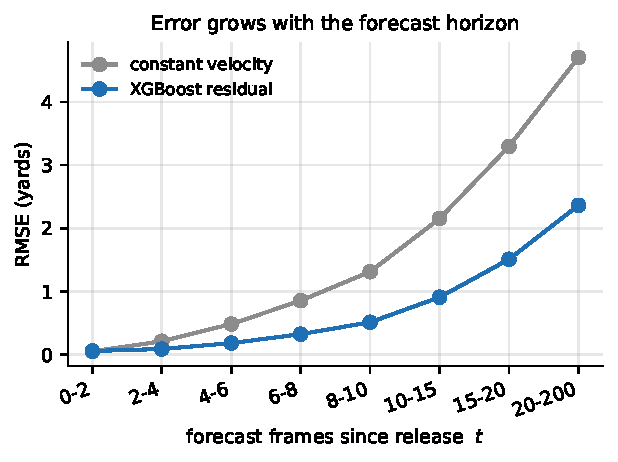
\includegraphics[width=0.62\linewidth]{figures/horizon.pdf}
\caption{RMSE by forecast step on held-out weeks. The learned corrector tracks the
trajectory closely for the first few frames and then diverges far more slowly than
pure extrapolation.}
\label{fig:horizon}
\end{figure}

\begin{table}[t]
\centering
\caption{RMSE (yards) by forecast step, held-out weeks 17--18.}
\label{tab:horizon}
\begin{tabular}{@{}rrrrr@{}}
\toprule
Forecast frames $t$ & rows & Constant velocity & XGBoost residual & Reduction \\
\midrule
0--2    & 10{,}076 & 0.053 & 0.060 & $-13\%$ \\
2--4    & 10{,}076 & 0.213 & 0.091 & $57\%$ \\
4--6    & 10{,}052 & 0.485 & 0.184 & $62\%$ \\
6--8    &  9{,}144 & 0.856 & 0.325 & $62\%$ \\
8--10   &  6{,}812 & 1.313 & 0.514 & $61\%$ \\
10--15  &  9{,}617 & 2.153 & 0.910 & $58\%$ \\
15--20  &  4{,}483 & 3.296 & 1.510 & $54\%$ \\
20--200 &  2{,}498 & 4.704 & 2.364 & $50\%$ \\
\bottomrule
\end{tabular}
\end{table}

Table~\ref{tab:role} and Figure~\ref{fig:role} split the same errors by player role
and release speed. Defensive coverage is roughly 60\% harder than the targeted
receiver at every setting, which is expected: the receiver runs a designed route
toward a known landing point, whereas coverage players react to a route they can only
partly anticipate. The corrector helps at every release speed and helps the harder
coverage group proportionally more.

\begin{table}[t]
\centering
\caption{RMSE (yards) by player role, held-out weeks 17--18.}
\label{tab:role}
\begin{tabular}{@{}lrrr@{}}
\toprule
Group & rows & Constant velocity & XGBoost residual \\
\midrule
Defensive coverage & 44{,}792 & 1.753 & 0.827 \\
Targeted receiver  & 17{,}966 & 1.339 & 0.514 \\
\midrule
All predicted players & 62{,}758 & 1.645 & 0.751 \\
\bottomrule
\end{tabular}
\end{table}

\begin{figure}[t]
\centering
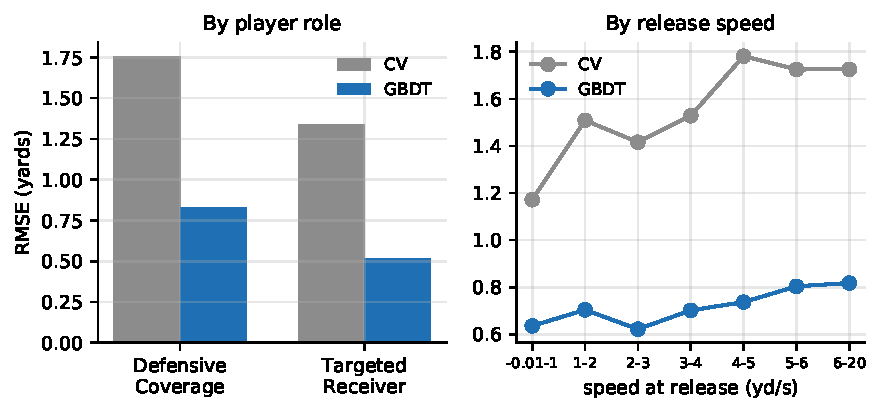
\includegraphics[width=0.86\linewidth]{figures/role_speed.pdf}
\caption{Error by player role and by release speed.}
\label{fig:role}
\end{figure}

Two further splits localize the residual error, shown in
Figure~\ref{fig:bdist}. Players far from the landing point are the hard cases: below
10 yards the error is about 0.354 yards, whereas beyond 30 yards it is 1.786, a
fivefold increase, while constant velocity degrades more gently. The model is being
asked to invent motion it cannot observe, and does so conservatively. Splitting the
error along and across the pass direction gives 0.786 and 0.714 yards respectively,
with mean residuals of $-0.029$ and $0.014$ yards. There is thus no systematic bias
left to correct; the remaining loss is variance, that is, genuine uncertainty about
route shape.

\begin{figure}[t]
\centering
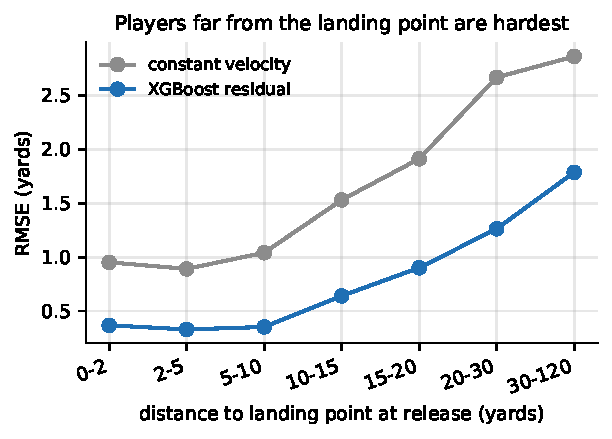
\includegraphics[width=0.62\linewidth]{figures/bdist.pdf}
\caption{Error against the player's distance from the landing point at release.}
\label{fig:bdist}
\end{figure}

\section{Targeted Ablations}
\label{sec:ablations}

The proposal specifies three ablations for the neural model. Because that model is
not yet trained, we run the analogous feature-group ablations on the boosted-tree
baseline, which tests the same questions in the same order of importance: whether
motion history matters, whether player interaction matters, and how much the supplied
landing geometry is worth. Table~\ref{tab:ablations} and Figure~\ref{fig:ablation}
report the results.

\begin{table}[t]
\centering
\caption{Feature-group ablations on Baseline 2, held-out weeks 17--18. The full row
is a separate fit under the ablation protocol, so it differs in the last digit from
Table~\ref{tab:headline}.}
\label{tab:ablations}
\begin{tabular}{@{}lrrr@{}}
\toprule
Variant & features & RMSE (yd) & $\Delta$ vs.\ full \\
\midrule
full model                        & 127 & 0.750 & -- \\
no interaction features           &  73 & 0.764 & $+0.014$ \\
short (5-frame) history only      &  97 & 0.772 & $+0.022$ \\
no history summaries              & 103 & 0.773 & $+0.023$ \\
neither history nor interaction   &  49 & 0.787 & $+0.037$ \\
no landing-point geometry         & 114 & 1.000 & $+0.250$ \\
\bottomrule
\end{tabular}
\end{table}

\begin{figure}[t]
\centering
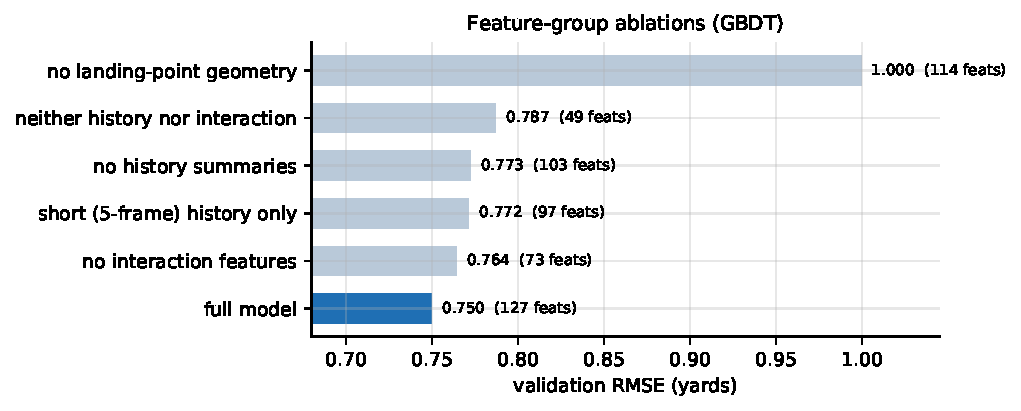
\includegraphics[width=0.66\linewidth]{figures/ablation.pdf}
\caption{Ablations ordered by validation RMSE. Every variant remains well below
constant velocity (1.645 yards); the informative comparison is against the full
model.}
\label{fig:ablation}
\end{figure}

Three findings follow, each with a design consequence for the temporal and interaction
model.

First, the landing point is the dominant signal. Removing it costs 0.250 yards
(1.000 against 0.750), by far the largest effect, and also widens the gap between
roles, because without a target to aim at the model cannot specialize. The neural
model must therefore receive landing-point geometry explicitly rather than learn it
from positions.

Second, interaction features help modestly and independently. Dropping all neighbour
and team-shape features costs 0.014 yards, and removing history and interaction
together costs 0.037, more than the sum of the two individually. This is the first
quantitative evidence for the interaction hypothesis behind the attention module, and
it also bounds how much a better interaction model can buy. We note that this
ablation is a single fit per variant, whereas the headline number carries a
three-seed spread of standard deviation 0.0015; the effect is about ten times that
spread, but it has not itself been estimated across seeds, so we treat the ordering
of the three history variants as unresolved.

Third, motion history is largely redundant beyond a short window. Keeping only the
5-frame summaries and discarding the 10- and 20-frame windows costs 0.022 yards, and
removing history summaries altogether costs 0.023. A recurrent encoder over the
history is therefore unlikely to justify itself through per-player motion alone; its
value, if any, must come from representing coordinated motion. This is a constraint
on the next milestone rather than a result about the neural model, which has not been
trained.

\section{Discussion and Limitations}
\label{sec:discussion}

The baselines answer the first half of our question. Recent motion alone is worth
1.645 yards, and a strong feature-based learner nearly halves that. The remaining
error is dominated by the long-horizon tail and by coverage players distant from the
landing point, both cases in which the future depends on intent that tracking does
not observe. That is the regime in which a learned interaction model could plausibly
help, and the ablations indicate that the ceiling on interaction-only gains is a few
hundredths of a yard unless the representation captures coordination better than
nearest-neighbour geometry does.

The limits of these findings should be stated plainly, because they bound any
comparison with the leaderboard. The landing point and horizon are given, so absolute
RMSE is not comparable to a system that must infer them at release. The 20-frame
history window is truncated for 13.7\% of plays, which have fewer than 20 observed
frames, while the 10-frame window is truncated for only 0.09\%; a further 1.1\% of
plays request more future frames than they have history frames. All are handled by
explicit masks rather than imputation, but they bound what the long windows can
contribute. Validation rests on two weeks of one season, so it carries a mild
distribution shift and considerable estimation noise on the long-horizon tail, and
because the metric pools over player-frames a handful of long plays carry
disproportionate weight in the aggregate. We therefore report per-play medians
alongside the pooled number above. Finally, the mock test files are unlabelled, so no
score on them is meaningful beyond format validity.

One design risk deserves to be on the record. The supplied landing point makes this a
conditional forecasting task, and a neural model that quietly re-encodes the landing
point may show gains attributable to that prior rather than to attention. The
no-landing-geometry ablation is our control for this, and we will keep it in the
final evaluation. Nothing in this stage required a GPU: the boosted-tree baseline
fits in about five minutes and evaluates in seconds, so the budget for the next
milestone should go to model and feature design rather than infrastructure.

\section{Work Plan}
\label{sec:plan}

Weeks 6--9 are complete. The remaining milestones are unchanged from the proposal.

\begin{center}
\begin{tabular}{@{}p{0.19\linewidth}p{0.76\linewidth}@{}}
\toprule
Course weeks & Planned milestone \\
\midrule
6--9 & Confirm the split, audit the data, implement both baselines, and submit the mid-term report in week 9. \\
10--12 & Implement the temporal and interaction model and select hyperparameters on validation data. \\
13--15 & Complete ablations and error analysis, freeze the configuration, and prepare the week-15 poster. \\
16--17 & Finalize held-out evaluation, document reproducibility, and submit the final report and implementation in week 17. \\
\bottomrule
\end{tabular}
\end{center}

For weeks 10--12 the model is a shared GRU encoder over each player's observed
history, a masked attention layer that mixes embeddings within the play with scores
conditioned on relative position, relative velocity, team, and role, and a shared MLP
mapping the result plus landing-point geometry and time features to a
constant-velocity correction as in Eq.~\eqref{eq:model}. All requested frames are
decoded in one shot from release-time information, exactly as the baselines do, so
that comparisons remain apples-to-apples. Three design choices follow directly from
the results above: keep the landing geometry as an explicit input, do not spend
capacity on long history windows, and target the interaction representation, which is
the only component whose ablation leaves room to improve. We will tune on weeks
17--18 under the same pooled metric, report three seeds with mean and standard
deviation, and repeat the proposal's three ablations, namely removing attention,
replacing the temporal encoder with a last-frame encoder, and removing the residual
connection, together with the landing-geometry control. If the neural model does not
beat 0.751 yards by a margin exceeding seed noise, we will report that outcome and
shift effort in weeks 13--15 toward error analysis and a stronger feature-based
reference.

\begin{thebibliography}{9}

\bibitem{competition}
NFL and Kaggle.
\newblock NFL Big Data Bowl 2026 -- Prediction: Overview and evaluation.
\newblock \url{https://www.kaggle.com/competitions/nfl-big-data-bowl-2026-prediction/overview}.

\bibitem{data}
NFL and Kaggle.
\newblock NFL Big Data Bowl 2026 -- Prediction: Data description.
\newblock \url{https://www.kaggle.com/competitions/nfl-big-data-bowl-2026-prediction/data}.

\bibitem{xgboost}
Tianqi Chen and Carlos Guestrin.
\newblock XGBoost: A scalable tree boosting system.
\newblock In \emph{Proceedings of ACM SIGKDD}, 2016.

\bibitem{gru}
Kyunghyun Cho, Bart van Merri\"enboer, Caglar Gulcehre, Dzmitry Bahdanau,
Fethi Bougares, Holger Schwenk, and Yoshua Bengio.
\newblock Learning phrase representations using RNN encoder--decoder for statistical machine translation.
\newblock In \emph{Proceedings of EMNLP}, 2014.

\bibitem{attention}
Ashish Vaswani, Noam Shazeer, Niki Parmar, Jakob Uszkoreit, Llion Jones,
Aidan N. Gomez, \L{}ukasz Kaiser, and Illia Polosukhin.
\newblock Attention is all you need.
\newblock In \emph{Advances in Neural Information Processing Systems}, 2017.

\end{thebibliography}
\end{document}
